\documentclass[aspectratio=169]{beamer}

\usepackage[utf8]{inputenc}
% \usepackage[portuguese]{babel}
\usepackage{graphicx}
\usepackage{tikz}
\usepackage{hyperref}
\usepackage{lipsum}
\usepackage{multicol}

\usepackage{./libs/solarized-light}

\usetheme{Luebeck}

\title{Data migration to Plone 5.2 and Volto}
\author{Rodrigo Ferreira de Souza}
\date{October, 2019}

\usebackgroundtemplate{%
    \tikz\node[opacity=0.2] {
        \vbox to \paperheight{
            \vspace{14mm}
            \vfil
            \hbox to \paperwidth{
                \hfil
                
\includegraphics[height=.6\paperheight]{./img/background.png}
                \hfil
            }
            \vfil
        }
    };
}

\hypersetup{
    colorlinks=true,
    linkcolor=cyan,
    filecolor=magenta,      
    urlcolor=blue,
}

\begin{document}

\maketitle

\AtBeginSection[] {
  \begin{frame}
    \frametitle{Where we are}
    % \begin{multicols}{2}
    % \setcounter{tocdepth}{1}
    \tableofcontents[currentsection]
    % \end{multicols}
  \end{frame}
}


\section{Knoledgements}
\subsection{Options to Migrate}
\begin{frame}
  \frametitle{Options to Migrate}

  \begin{columns}
    \column{.5\textwidth}
    \begin{itemize}
      \item Plone 4.3 $\rightarrow$ Plone 5+
      \begin{itemize}
        \item \href{https://github.com/collective/collective.transmogrifier}{Collective Transmogrifier} \pause
      \end{itemize}
      \item Plone 5.1 $\rightarrow$ Plone 5.2+
      \begin{itemize}
        \item \href{https://docs.plone.org/manage/upgrading/version_specific_migration/upgrade_zodb_to_python3.html}{Migrate a ZODB from Python 2.7 to Python 3} \pause
        \item \href{https://github.com/collective/collective.transmogrifier}{Collective Transmogrifier} \pause
      \end{itemize}
    \end{itemize}
    \column{.5\textwidth}
    \begin{figure}
      
\includegraphics[height=.5\textheight]{./img/002_-_transmogrifier.png}
      \caption{A transmogrifier is fictional device used for transforming one object into another object. The term was coined by Bill Waterson of Calvin and Hobbes fame.}
    \end{figure}
  \end{columns}
\end{frame}

\subsection{Why we use Transmogrifier?}
\begin{frame}
  \frametitle{Why we use Transmogrifier?}

  \begin{columns}
    \column{.5\textwidth}
    \begin{itemize}
      \item Have many generic Pipelines available for common cases \pause
      \item Flexibility to deal with different use cases \pause
      \item Briliant way to use Iterator Design Pattern! \pause
    \end{itemize}

    \column{.5\textwidth}
    \begin{figure}
      \includegraphics[width=\textwidth]{./img/001_-_Transmogrify_diagram.png}
      \caption{Transmogrify Diagram}
    \end{figure}
  \end{columns}
\end{frame}

\begin{frame}
  \frametitle{Why we use Transmogrifier?}

  \begin{columns}
    \column{.5\textwidth}
    \begin{itemize}
      \item Have many generic Pipelines available for common cases
      \item Flexibility to deal with different use cases
      \item Briliant way to use Iterator Design Pattern!
    \end{itemize}

    \column{.5\textwidth}
    \begin{figure}
      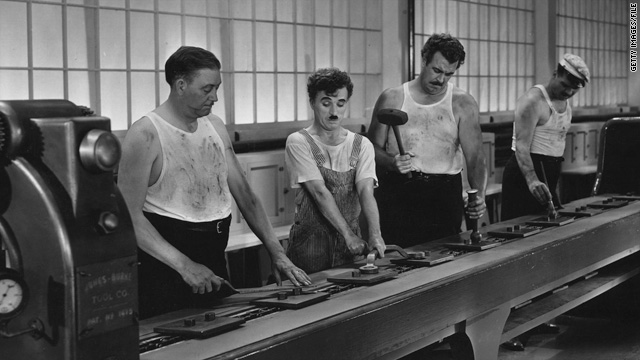
\includegraphics[width=\textwidth]{./img/001_-_modern_times.jpg}
      \caption{Modern Times -- Production line}
    \end{figure}
  \end{columns}
\end{frame}

\section{Use cases}
\subsection{Large University}
\begin{frame}
  \frametitle{Large University}
  \begin{figure}
    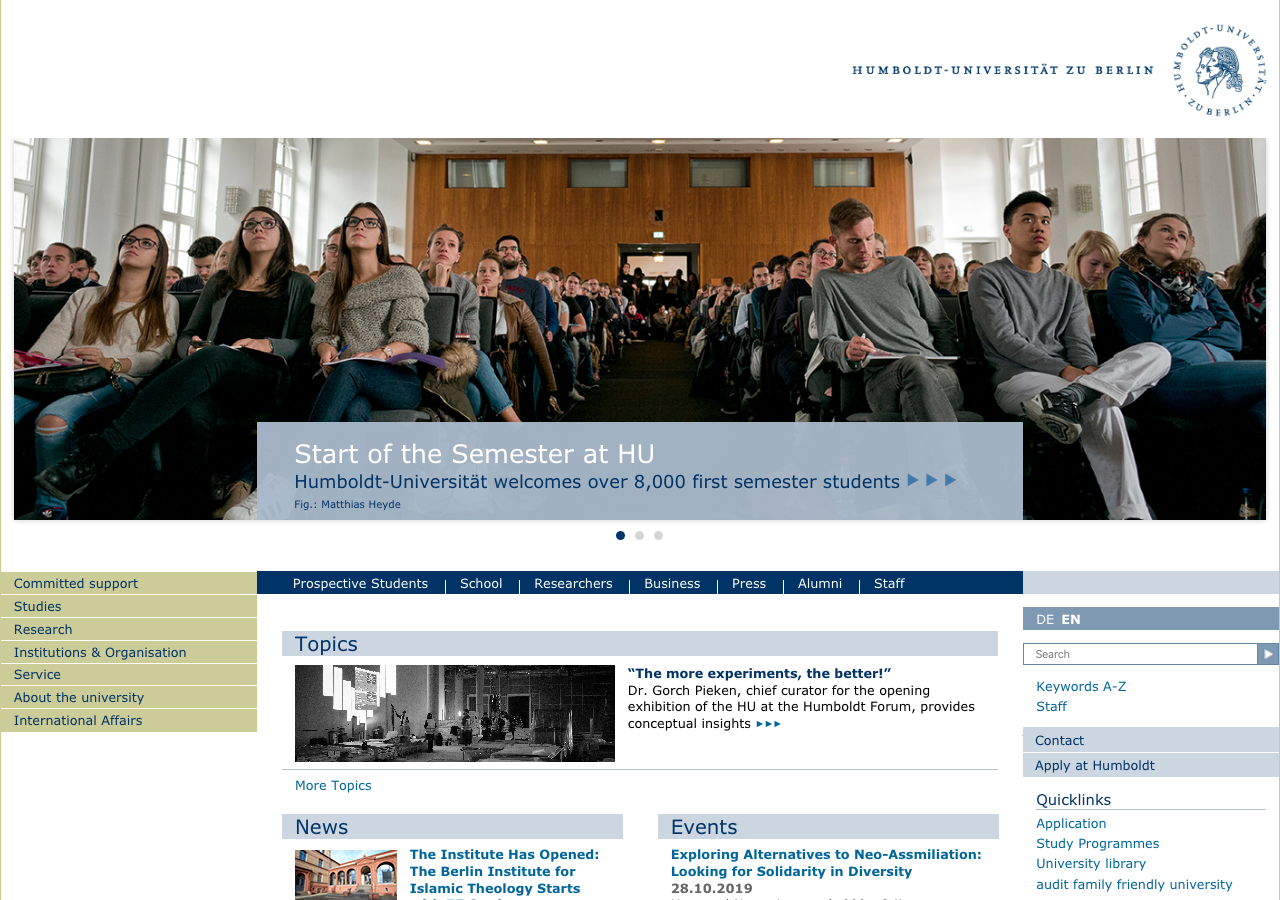
\includegraphics[height=.7\textheight]{./img/003_-_huberlin.png}
    \caption{Humboldt-Universität zu Berlin}
  \end{figure}
\end{frame}

\subsection{High-profile government client}
\begin{frame}
  \frametitle{High-profile government client}
  \begin{figure}
    
\includegraphics[height=.7\textheight]{./img/004_-_brh.jpg}
    \caption{Bundes rechnungshof}
  \end{figure}
\end{frame}

\subsection{One of the largest research institutions in Germanpngpngy}
\begin{frame}
  \frametitle{One of the largest research institutions in Germany}
  \begin{figure}
    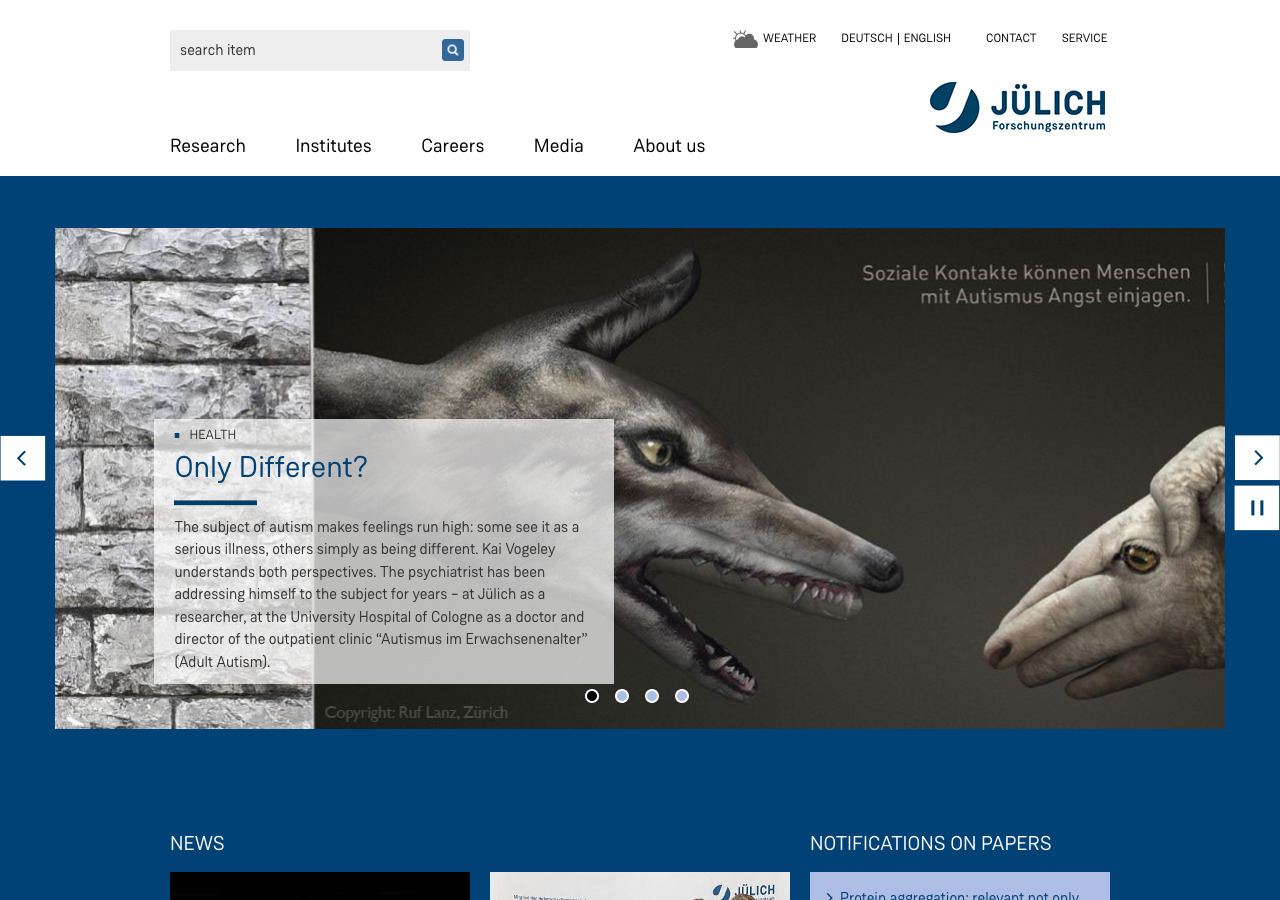
\includegraphics[height=.7\textheight]{./img/005_-_fzj.jpg}
    \caption{Forschungszentrum Jülich -- Intranet}
  \end{figure}
\end{frame}

\section{The challendge}
\subsection{The challendge}
\begin{frame}
  \frametitle{The challendge}
  \begin{itemize}
    \item Plone 4.3 $\rightarrow$ Plone 5+
    \begin{itemize}
      \item \href{https://plone.com/try-plone.html}{Transmogrifier}
    \end{itemize}
    \item Plone 5.1 $\rightarrow$ Plone 5.2+
    \begin{itemize}
      \item Transmogrifier
      \item Database Migration
    \end{itemize}
  \end{itemize}
\end{frame}


% \subsection{Criar páginas}
% \begin{frame}
%     \frametitle{Criar páginas}
%     \begin{figure}
%         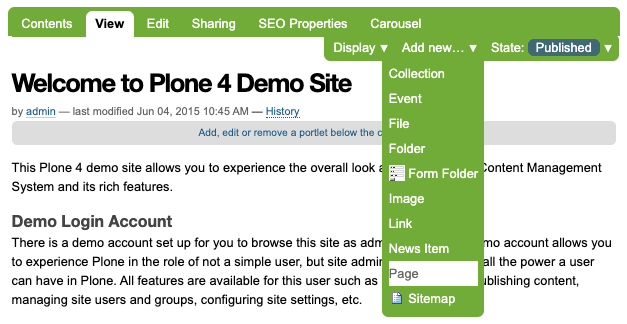
\includegraphics[width=.7\textwidth]{./img/001-002_-_create_page.png}
%         \caption{Menu para criação de páginas}
%     \end{figure}
% \end{frame}

% \subsection{Adicionar texto}
% \begin{frame}
%     \frametitle{Adicionar texto}
%     \begin{figure}
%         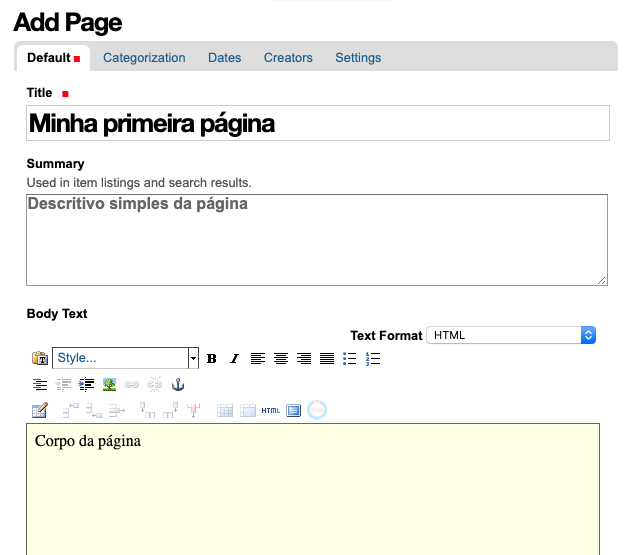
\includegraphics[height=.7\textheight]{./img/001-003_-_adicionar_texto.png}
%         \caption{Redigindo uma página}
%     \end{figure}
% \end{frame}

% \subsection{Publicar}
% \begin{frame}
%     \frametitle{Publicar}
%     \begin{figure}
%         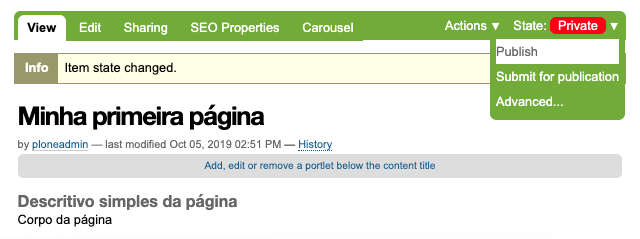
\includegraphics[width=.7\textwidth]{./img/001-004_-_publicar_pagina.png}
%         \caption{Workflow simples - Publicar página}
%     \end{figure}
% \end{frame}

% \subsection{Página publicada}
% \begin{frame}
%     \frametitle{Página publicada}
%     \begin{figure}
%         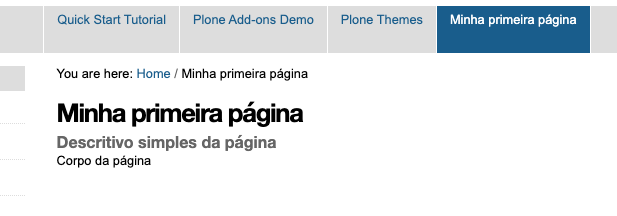
\includegraphics[width=.7\textwidth]{./img/001-005_-_pagina_publicada.png}
%         \caption{Resultado final}
%     \end{figure}
% \end{frame}

% \subsection{portlets}
% \begin{frame}
%     \frametitle{portlets}
%     \begin{figure}
%         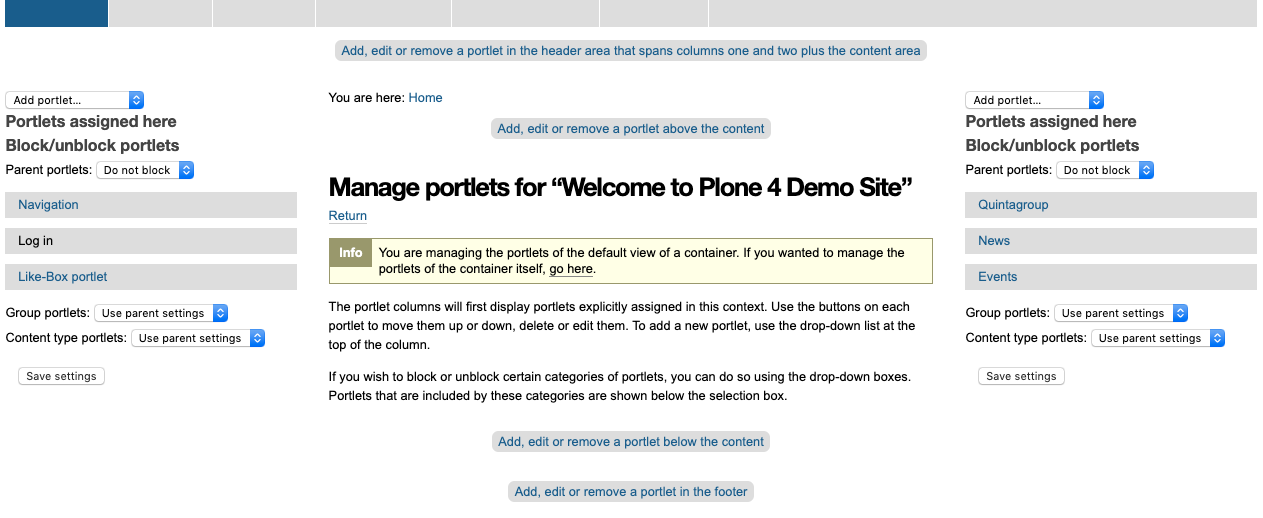
\includegraphics[width=.7\textwidth]{./img/001-006_-_portlets.png}
%         \caption{gerenciador de portlets}
%     \end{figure}
% \end{frame}

% \section{IDG - Identidade Digital de Governo}
% \subsection{Portal Padrão}
% \begin{frame}
%     \frametitle{Portal Padrão}
%     \begin{figure}
%         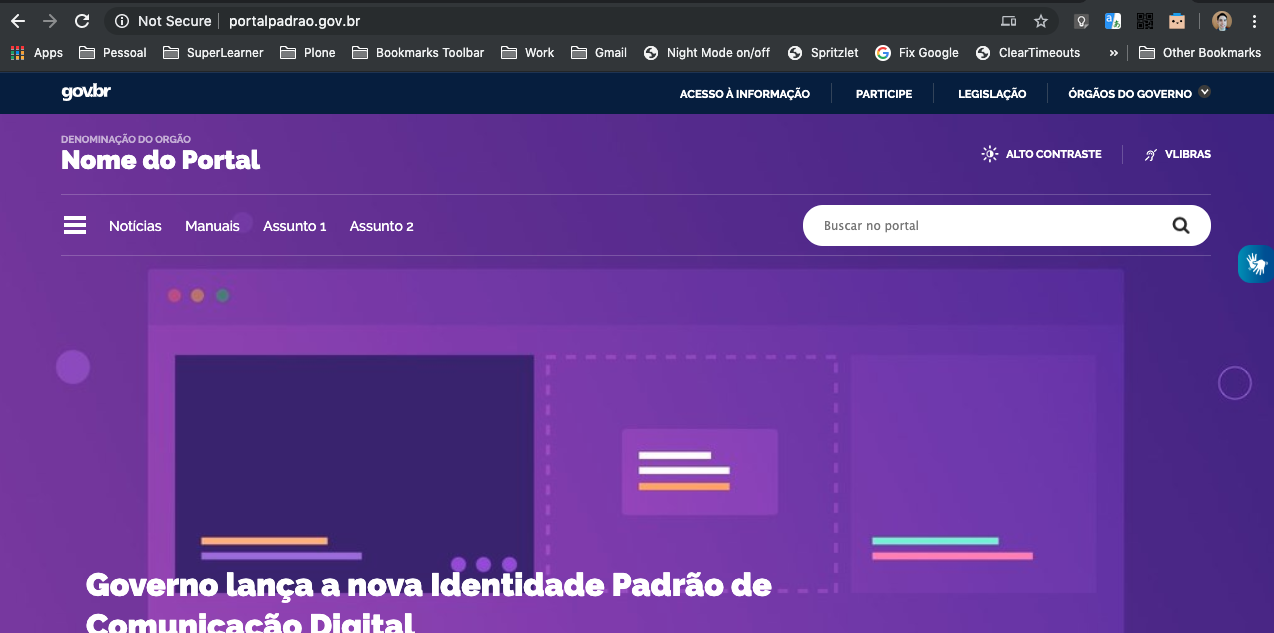
\includegraphics[width=.7\textwidth]{./img/001-007_-_portal_padrao.png}
%         \caption{\href{http://www.portalpadrao.gov.br/}{Site do Portal Padrão}}
%     \end{figure}
% \end{frame}

% \subsection{Características}
% \begin{frame}
%     \frametitle{Características}
%     \begin{columns}
%         \column{.4\textwidth}
%         Temas que seguem \href{http://emag.governoeletronico.gov.br/}{eMAG}
%         \begin{itemize}
%             \item \href{https://github.com/plonegovbr/brasil.gov.portal}{brasil.gov.portal} \pause
%             \item \href{https://github.com/plonegovbr/brasil.gov.temas}{brasil.gov.temas} \pause
%             \item \href{https://github.com/plonegovbr/brasil.gov.portlets}{brasil.gov.portlets} \pause
%             \item \href{https://github.com/plonegovbr/brasil.gov.tiles}{brasil.gov.tiles} \pause
%             \item \href{https://github.com/plonegovbr/brasil.gov.barra}{brasil.gov.barra} \pause
%             \item \href{https://github.com/plonegovbr/brasil.gov.agenda}{brasil.gov.agenda} \pause
%             \item \href{https://github.com/plonegovbr/brasil.gov.vcge}{brasil.gov.vcge}
%         \end{itemize}

%         \column{.3\textwidth}
%         Complementos
%         \begin{itemize}
%             \item \href{https://github.com/collective/collective.cover}{Cover} \pause
%             \item \href{https://github.com/collective/collective.fingerpointing}{Finger Pointing} \pause
%             \item \href{https://github.com/collective/collective.lazysizes}{Lazy Sizes} \pause
%             \item \href{https://github.com/collective/collective.liveblog}{Live Blog} \pause
%             \item \href{https://github.com/collective/collective.nitf}{NITF} \pause
%         \end{itemize}
%         \column{.3\textwidth}
%         \begin{itemize}
%             \item \href{https://github.com/collective/collective.polls}{Polls} \pause
%             \item \href{https://github.com/collective/collective.upload}{Upload} \pause
%             \item \href{https://github.com/collective/sc.social.likes}{Likes} \pause
%             \item \href{https://github.com/collective/sc.photogallery}{Photogallery} \pause
%             \item \href{https://github.com/collective/sc.embedder}{Embedder}
%         \end{itemize}
%     \end{columns}
% \end{frame}

% \subsection{Cover}
% \begin{frame}
%     \frametitle{Cover}
%     \begin{figure}
%         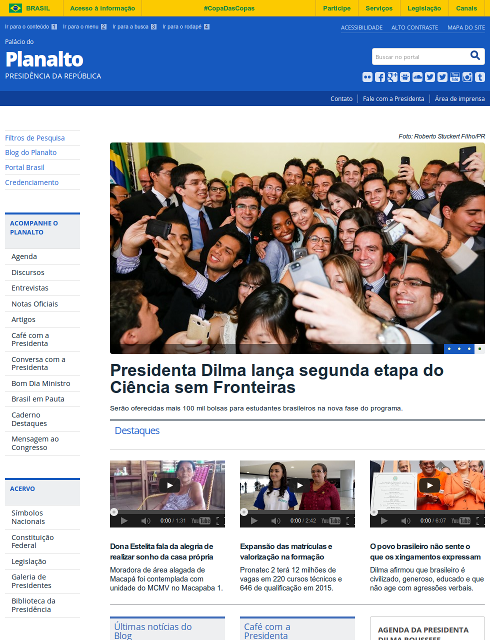
\includegraphics[height=.7\textheight]{./img/001-008_-_cover.png}
%         \caption{\href{https://github.com/collective/collective.cover/blob/master/docs/end-user.rst}{Tutorial para usuários}}
%     \end{figure}
% \end{frame}

% \subsection{Upload}
% \begin{frame}
%     \frametitle{Upload}
%     \begin{figure}
%         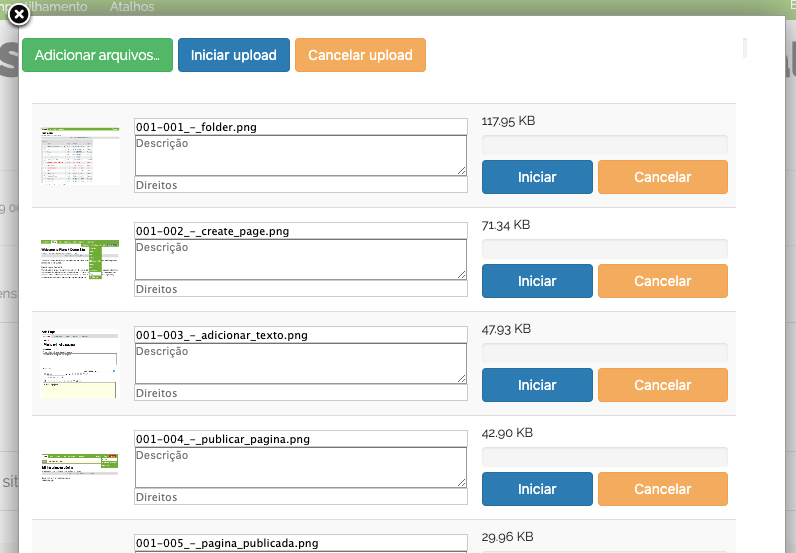
\includegraphics[height=.7\textheight]{./img/001-009_-_upload.png}
%         \caption{\href{https://github.com/collective/collective.upload}{Collective Upload}}
%     \end{figure}
% \end{frame}

% \subsection{NITF e Likes}
% \begin{frame}
%     \frametitle{NITF e Likes}
%     \begin{figure}
%         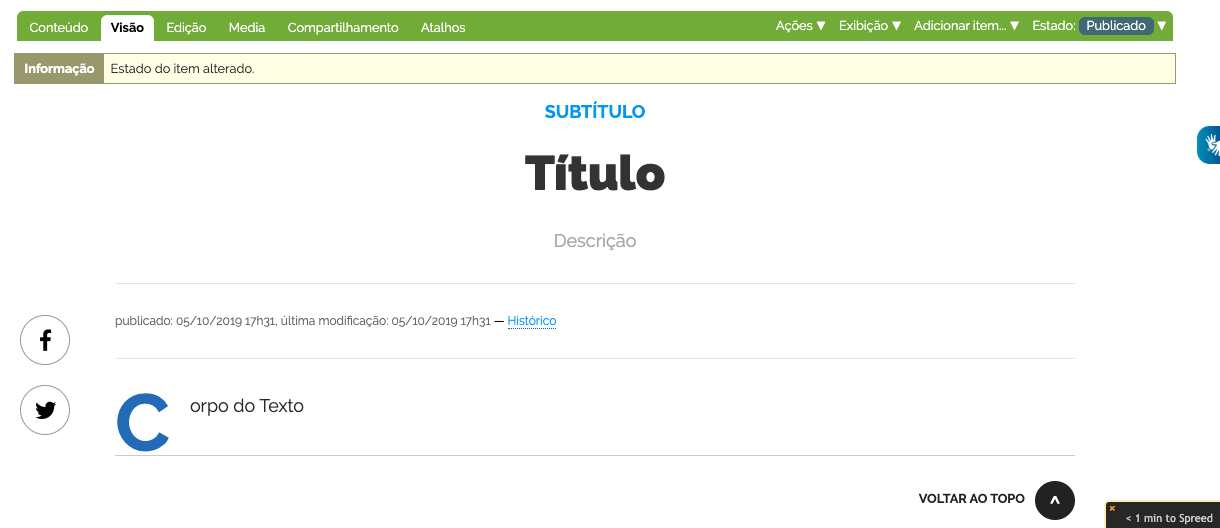
\includegraphics[height=.6\textheight]{./img/001-010_-_nitf_e_likes.png}
%         \caption{\href{https://github.com/collective/collective.nitf}{NITF} e \href{https://github.com/collective/sc.social.likes}{Likes}}
%     \end{figure}
% \end{frame}

% \subsection{Embedder}
% \begin{frame}
%     \frametitle{Embedder}
%     \begin{figure}
%         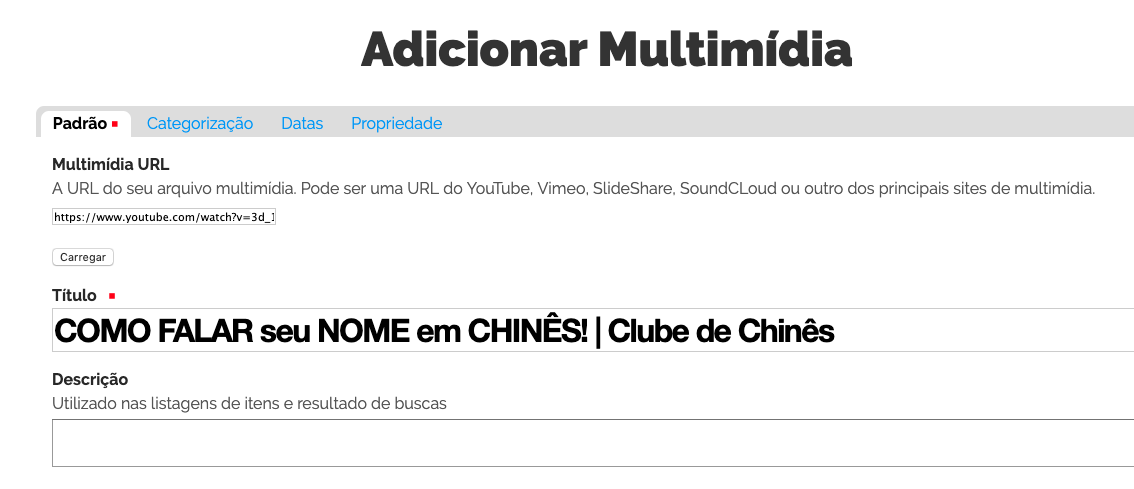
\includegraphics[height=.6\textheight]{./img/001-011_-_embedder.png}
%         \caption{\href{https://github.com/collective/sc.embedder}{Embedder}}
%     \end{figure}
% \end{frame}

% \subsection{Agenda}
% \begin{frame}
%     \frametitle{Agenda}
%     \begin{figure}
%         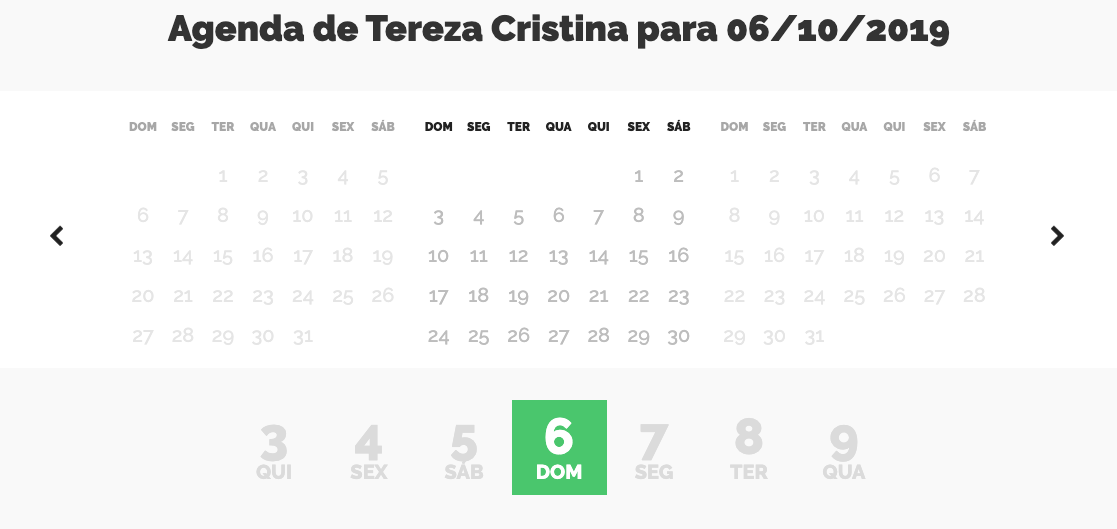
\includegraphics[height=.6\textheight]{./img/001-012_-_agenda.png}
%         \caption{\href{https://github.com/plonegovbr/brasil.gov.agenda}{Agenda}}
%     \end{figure}
% \end{frame}

% \section{Columns example}
% \subsection{Columns example}
% \begin{frame}
%     \frametitle{Columns example}
%     \begin{columns}
%         \column{.5\textwidth}
%         \lipsum[1][1-4]

%         \column{.5\textwidth}
%         \lipsum[2][1-4]
%     \end{columns}
% \end{frame}

% \section{Code example}
% \subsection{Code example}
% \begin{frame}[fragile]
%     \frametitle{Code example}
%     \begin{lstlisting}[language=python]
% @implementer(IBlocksTransformEnabled)
% class View(BrowserView):

%     """Default view, a compose page."""

%     index = ViewPageTemplateFile(
%         'templates/view.pt')

%     def __call__(self):
%         # forbid image indexing as scales are volatile
%         self.request.RESPONSE.setHeader(
%             'X-Robots-Tag', 'noimageindex')
%         return self.index()
%     \end{lstlisting}
% \end{frame}

\end{document}
